\documentclass{article}
\usepackage[utf8]{inputenc}
\usepackage{graphicx}

\title{Core Project Document}
\author{Boyd Verdoorn, Luuk de Niet, Jesper Spillenaar Bilgen\\ Rense Wisse, Thomas de Boer\\ \\Group 4: Pico Bello B.V.}
\date{12-11-2014}


\begin{document}
	\maketitle
	\begin{figure}[ht!]
		\centering
		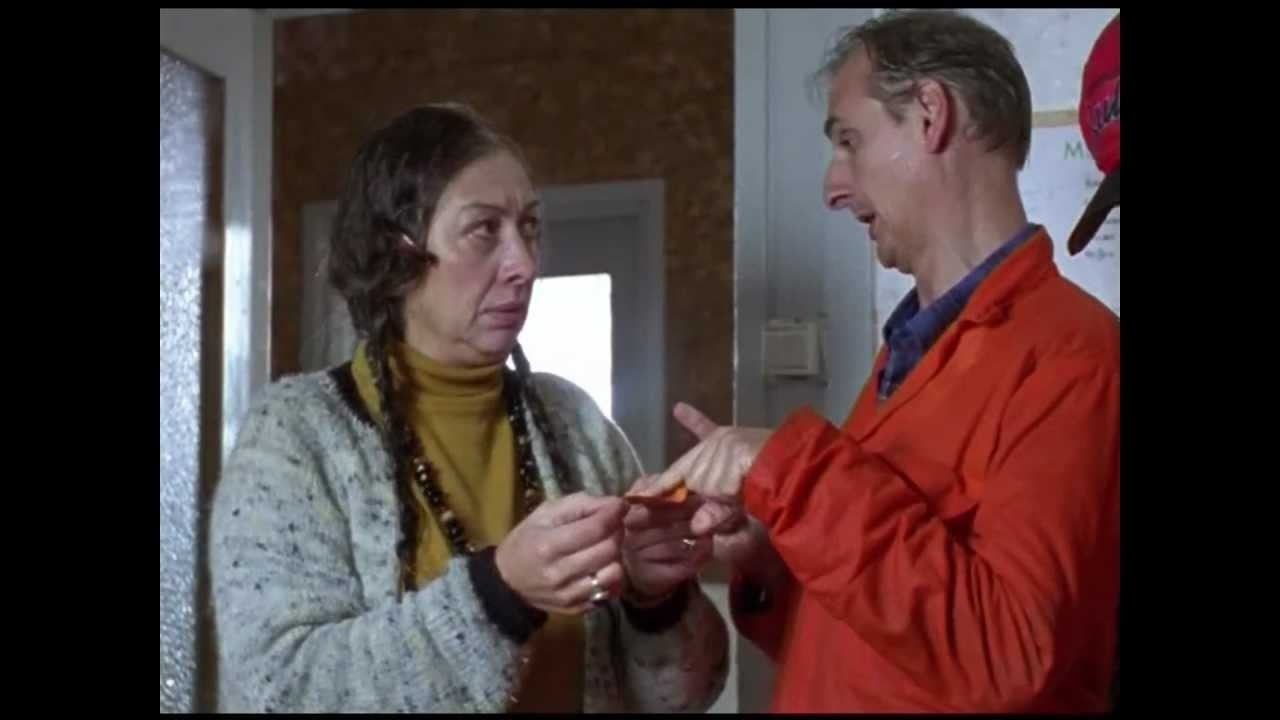
\includegraphics[width=120mm]{Front.jpg}
	\end{figure}
	\newpage

	\section{Summary}
		The game is based around a single story of a murder case. The story is told through different perpectives, each with their own destinctive gameplay and design. The story is told three times in total, each time giving more information about the murder. There are three roles: Detective, Journalist, and a family member. The game concludes in a finale, where, depending on the choices of the player, the killer is apprehended. The game is a sort of 'first person investigation' and is played by walking around in the scene with the keys and collecting evidence by clicking on different objects to investigate them.

	\section{Theme}
		You only get one story.
		There is only one story, but you get to see it on different levels and depending on your play style you get to see different things.

	\section{Target Audience}
		Our Target Audience is casual to midrange gamer, who is interested in an story based interactive experience. The age group is Teen to Adult. The target platform is PC, but we want to explore the possibility of expanding to mobile platforms as well, such as iOS and Android.

	\section{The Team}
		Group 4: Pico Bello B.V. consists of five team members.\\
				\textbf{Thomas de Boer}, Game Designer. 4172760 - t.w.j.deboer@student.tudelft.nl\\
		\textbf{Luuk de Niet}, Lead Artist. 4139658 - l.f.deniet93@gmail.com\\
		\textbf{Boyd Verdoorn}, Lead Programmer. 4209346 - b.c.verdoorn@student.tudelft.nl\\
		\textbf{Rense Wisse}, World Builder. 4230027 - r.r.wisse@student.tudelft.nl\\
		\textbf{Jesper Spillenaar Bilgen}, Producer. 4147405 - jesper\_sb\_91@hotmail.com

	\section{Schedule}
		We will adhere to the Schedule as given in the assignment.

	\section{GitHub}
		We use GitHub for our assets. The account EWI3620TU has been added to our repository. The Repo is private an can only be accessed by collaborators. If there are any problems, please contact Thomas de Boer. \\
		\\
		URL: https://github.com/twjdeboer/4-AwesomeSpel

	\newpage
	\section{Components}
		\subsection{Computer Graphics - Luuk and Thomas $18 \star$}
			\begin{itemize}
				\item \textbf{3D Models}\\
					\underline{3D Models} $\star \star \star$ We will use 3D models for interactive objects and clutter. We are giving this 3 starts because our game need many different models to create the city, players and all evidence. We also created procedural models withing blender by adding drivers, which creates an extra difficulty. Besides all of that, none of us had ever worked with Blender which makes this an extra difficult task for us.\\
					\underline{3D Animated Models} $\star \star$  We will use 3D animated models for the player and NPCs.\\
					\underline{Procedural Meshes} $\star \star \star$  the street map and some important buildings will be recurring objects. All buildings in the city that are of less importance will be procedurally generated by a unity script.
				\item \textbf{Textures}\\
					\underline{Textures} $\star$ We will use differnt textures for game objects.\\
					\underline{Bump mapping/grime} $\star \star$ We will use texture overlays to make objects dirty and unique.
				\item \textbf{Special FX \& Juiciness}\\
					\underline{Sound Effects} $\star$ Sound effects will be used to immerge the gamer more in the action.\\
					\underline{Camera Shakes} $\star$ Camera shakes will emphasize loud noise or vibrations.\\
					\underline{Particle System} $\star$ We will use Particles to simulate different environmental factors, such as rain or smoke.
				\item \textbf{Rendering}\\
					\underline{Light and Shadows} $\star$  We will use many diffents ways of lighting to create shadows where the player can hide from onlookers. This has only one star because it doen't implement the hiding part yet. This will be integrated in the conciousness of enemies.
				\item \textbf{User Interface}\\
					\underline{Start/Pauze/Quit} $\star$ These screens will start, pauze or quit the game.\\
					\underline{Option} $\star$ Music volume and control mapping\\
					\underline{Credits} $\star$ Show how awesome we are and give credit where due.
			\end{itemize}
		\subsection{Artificial Intelligence - Jesper $9 \star$}
			\underline{Some Consciousness in enemies} $\star \star \star$ Enemies will be less likely to detect you in when walking in shadows. They will pursue you when they see you. This implements the likelyhood of an enemy seein you and the way it will chace you.\\
			\underline{Use a NavMesh, Pathfinding} $\star \star$ Enemy Pathfinding.\\
			\underline{Implement a Neural Network} $\star \star \star \star$ A neural network will be used to find out how close you are to finding the right killer according to the evidence you have found. We will make a list of examples with combinations of found evidence and train the network with this. The output of the network will state how close you are to finding the killer and according to this you will be placed close or far away from the killer in the final scene and thus making it easier or harder to catch the killer in th final scene.
		\subsection{Web \& Database - Rense $8 \star$}
			\underline{Collect playthrough data} $\star \star$ We will save data (time you have been playing, collected items, position etc.) for the game. \\
			\underline{Store data on web server} $\star \star$ Store the data stated above. \\
			\underline{Visualize data on web server} $\star \star$ Show statistics. \\
			\underline{Collect and show highscores} $\star \star$ Highscores are available from a web page. \\
			\textit{Optional:} \underline{Save and share game states} $\star \star \star$ on social networking sites.
		\subsection{Programming - Boyd $12 \star$}
			\begin{itemize}
				\item \textbf{Game Mechanics}\\
					\underline{Procedurally placing Evidence} $\star \star \star$ The evidence of importance already exists and will be placed randomly in the environment, but extra object that looks like evidence will be procedurally generated and place to create distractions. This will however not have impact on the game play.\\
					\underline{Race against the Clock} $\star$ Some evidence will fade with time. Hurry up and go get it, you lazy bum.
				\item \textbf{Game Loop}\\
					\underline{Fps independent} $\star \star$ The game will run the same speed, independent of frame rate.
					\underline{Fast Forward} $\star$ Skip conversations you already know.
				\item \textbf{Physics}\\
					\underline{Collision Checking} $\star$ Check if there's a wall in the way.\\
					\underline{Movement} $\star$ Make sure the player moves using animations and bone structur. (Optinal extra star for running)\\
					\underline{Interaction with environment} $\star \star$ The player can klick on objects that ar lying around and is able to pick up important evidence.\\
					\underline{Conversation interface} $\star$ When clicking on object this will show what the possibillities are with this object. you can click on whatever you want to do with the object and keep playing.
			\end{itemize}

			\subsection*{Total: 47$\star$}

			




\end{document}